\documentclass[letter,12pt]{article}
\usepackage[utf8]{inputenc}
\usepackage[T1]{fontenc}
\usepackage[margin=1cm]{geometry}
\usepackage[makeroom]{cancel}
\usepackage[export]{adjustbox}
\usepackage[spanish]{babel}
\usepackage{graphicx}
\usepackage[
backend=biber,
style=ieee,
minnames=1,
maxcitenames=2, maxbibnames=6
]{biblatex}
\DefineBibliographyStrings{spanish}{%
	url = {[En línea]. Disponible en:},
}
\addbibresource{bibliography.bib}
%\usepackage[none]{hyphenat}
\usepackage{multicol,graphicx,fancyhdr,eso-pic,url,float,lmodern,listings,times,textcomp,amsthm,amsmath,amssymb,mathptmx,dsfont,color,colortbl,sidecap,xspace,epic,eepic,anysize,setspace,hyperref,pdflscape,subfigure,gensymb,siunitx,caption,subcaption,wrapfig,enumitem}

% Python SQL C++ HTML Matlab
\lstset{
	language=C,
	basicstyle=\ttfamily\small,
	numbers=left,
	numberstyle=\tiny,
	numbersep=5pt,
	showspaces=false,
	showstringspaces=false,
	breaklines=true,
}
\renewcommand{\lstlistingname}{Código}
\marginsize{2cm}{2cm}{2cm}{2cm}

\rhead{Ingeniería Civil en Informática}
\rfoot{Universidad de Los Lagos}
\lfoot{M. Toro, A. Ibáñez}
\renewcommand{\headrulewidth}{0.5pt}
\renewcommand{\footrulewidth}{0.5pt}
\pagestyle{fancy} 

\begin{document}
	\begin{figure}
		
\includegraphics[width=0.3\textwidth, left]{figures/download.png}
	\end{figure}
	\setlength{\unitlength}{1 cm} 
	\title{\scshape\Huge{Tarea 2}\\\vspace{0.5cm}
		\Large \textbf{Casos de Alcaldes Fraudulentos}\\\vspace{2cm}
		\Large Ingeniería Civil en Informática\\\vspace{1cm}
		\Large Contabilidad y Costos\\\vspace{2cm}}
	
	\author{
		Matias Johan Toro Núñez\\
		matiasjohan.toro@alumnos.ulagos.cl \\\\
		Alvaro Benjamín Ibáñez Cisternas\\
		alvarobenjamin.@alumnos.ulagos.cl
		%\and
		%otro\\
		%otro.ulagos\\\\
		%otro\\
		%otro.ulagos
	\vspace{3cm}}
	
	\date{25/11/2024}
	\maketitle
	\thispagestyle{empty}
	\clearpage
	\setcounter{page}{1}
	
	\pagenumbering{Roman}
	\tableofcontents
	\newpage
	%\listoffigures
	%\newpage
	%\listoftables
	%\newpage
	%\lstlistoflistings
	%\newpage
	
	\pagenumbering{arabic}
	
	\section{Primer Caso\\}
		Margarita Osorio, ex-alcaldesa independiente de la comuna de Nogales, se encuentra en el centro de una polémica tras ser formalizada por el delito de estafa. Su gestión como autoridad municipal quedó bajo cuestionamiento luego de conocerse denuncias que involucraban defraudaciones económicas a familias de escasos recursos. Actualmente, enfrenta arresto domiciliario nocturno y arraigo nacional.\cite{margarita1}\\
	\begin{wrapfigure}{r}{0.4\textwidth}
		\centering
		
\includegraphics[width=0.4\textwidth]{figures/margarita-osorio}
	\end{wrapfigure}
	La Fiscalía presentó antecedentes que indican que Osorio, junto a otros dos imputados, implementó un esquema fraudulento para estafar a familias vulnerables y de medianos ingresos. Bajo la promesa de facilitar el acceso a la casa propia, solicitaban pagos de diversas sumas de dinero. Según los registros oficiales, la trama habría defraudado a dos comités de vivienda en Nogales y El Melón, generando un perjuicio económico total de aproximadamente 173 millones de pesos. Muchas familias de bajos recursos entregaron aportes iniciales superior a \$100.000 y continuamente fueron incrementando pidiendo más y más. Sin embargo, nunca se dio evidencias de algún progreso con lo planeado. Bajo investigaciones, el lugar determinado para construir las casas prometidas, no existía evidencias de trabajo en el lugar. Después de un tiempo, en el terreno se instalaron paneles solares. Mega en investigación habló con el dueño del terreno, el cual indicó que no había trato con la comuna en relación con los hogares prometidos. \cite{margarita2}\\
	Margarita Osorio ha rechazado las acusaciones y calificó el proceso como una “campaña del terror” en su contra. Con este argumento, la alcaldesa intentando desmentir las acusaciones, busca jugar un rol de victima, sugiriendo que se trata de una estrategia política para desprestigiarla.\cite{margarita3}\\\\
	Además de estas acusaciones,  también se le acusó de maltrato y acoso laboral a funcionarios del municipio. En el mes de abril del presente año, fue acusada de estar apostando, incumpliendo su arresto domiciliario y además la ley 19995 sobre la incapacidad de apostar que tienen los funcionarios públicos y municipales.
	
	
	\subsection{Análisis del caso\\}
	\subsubsection{Implicancias del caso}
	El caso de Margarita Osorio refleja la fragilidad institucional y la vulnerabilidad de los grupos sociales más desprotegidos frente a posibles abusos de poder. Los montos y la naturaleza de las denuncias evidencian una seria brecha en la ética pública que afecta directamente la confianza de los ciudadanos en sus autoridades locales. Esto se ve evidencia en sus conductas, las cuales no son de destacar en un alcalde. Es recurrente su lenguaje informal, siendo esto el menor de los problemas, puesto que en varias ocasiones ha llegado a proferir ofensas a nogalinos (residentes de nogales) y también a periodista o gente externa.\\
	Fuera de su actitud despreciable por muchos, realiza actos humanitarios y sociales en la comuna, lo que le ha traído reconocimiento por parte de los residentes del sector y ha motivado a su postulación a la alcaldía nuevamente.
	
	\subsubsection{Estado actual del acusado/a}
	Actualmente, Margarita Osorio enfrenta arresto domiciliario nocturno, el cual anteriormente había sido total y arraigo nacional, medidas decretadas por el Juzgado de Garantía de La Ligua. Estas sanciones provisionales estarán vigentes mientras avanza la investigación sobre su participación en el esquema de estafa. Sin embargo, aún no se encuentran pruebas contundentes para condenarla, aunque claramente se evidencia una falta clara en su compromiso con la gente que les prometió un hogar. Como mencionamos más arriba, este año se dieron a cabo las elecciones municipales, donde Margarita, decidió postularse nuevamente. Eso no es lo más sorprendente, sino que estuvo a pocos votos de quedarse nuevamente como la alcaldesa de nogales a pesar de las acusaciones en su contra. Como se puede ver en la siguiente imagen \ref{votacion}.
	\begin{figure}[H]
		\centering
		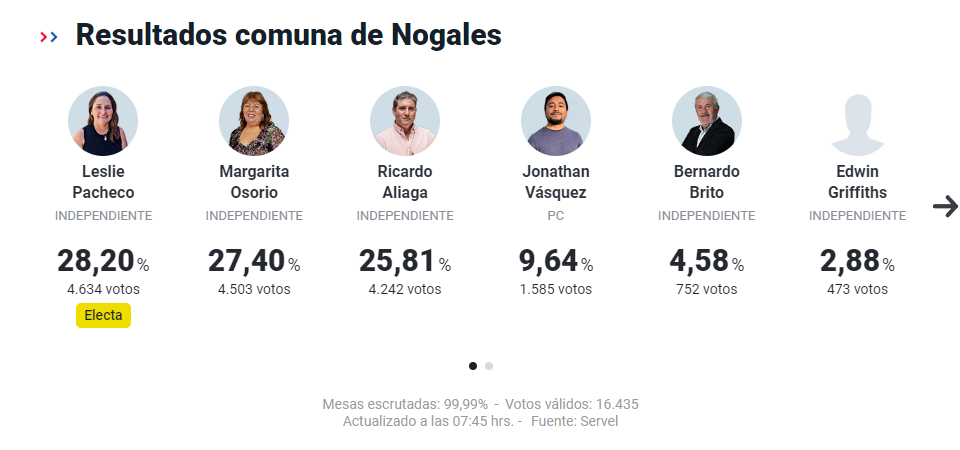
\includegraphics[width=1\textwidth]{figures/votaciones}
		\caption{Votaciones finales comuna de Nogales}\label{votacion}
	\end{figure}
	
	\subsubsection{Declaraciones}
	La alcaldesa Margarita Osorio defendió su posición rechazando las acusaciones en su contra. Afirmó que está a la espera de los resultados del proceso judicial y calificó las denuncias como injustificadas. Concretamente, expresó que considera que las imputaciones forman parte de una estrategia para dañar su reputación. Su postura, aunque contundente, no presentó pruebas claras que refuten las acusaciones presentadas por la Fiscalía. Además, siempre se justificó con dichos informales o comentarios fuera de lugar, incluso citando a Dios para justificar sus conductas.
	
	\section{Segundo Caso\\}
	\begin{wrapfigure}{l}{0.3\textwidth}
		\centering
		
\includegraphics[width=0.3\textwidth]{figures/oscar cortes}
	\end{wrapfigure}
	Óscar Cortés, ex-alcalde de Nogales, fue condenado por fraude al fisco debido a la utilización indebida de fondos públicos. Los hechos ocurrieron entre 2011 y 2013 y estuvieron relacionados con propaganda política financiada con recursos del municipio de la provincia de Quillota. Su condena incluye cinco años de libertad vigilada, el pago de \$221 millones, una multa mensual de 8 UTM, y la inhabilitación absoluta para ocupar cargos públicos.
	La Fiscalía estableció que Cortés, junto a tres directivos municipales, utilizó fondos públicos de manera ilícita, desviándolos hacia actividades de propaganda política. Este caso, que involucró una suma significativa de recursos públicos, fue denunciado como un acto de corrupción que traicionó la confianza de la comunidad.\cite{oscar1}
	
	\subsection{Análisis del caso\\}
	\subsubsection{Implicancias del caso}
	El caso de Óscar Cortés representa una violación grave a los principios de probidad administrativa, al involucrar el uso de fondos públicos para fines personales y políticos. Este tipo de actos generan un daño profundo a la confianza de los ciudadanos en sus líderes locales y perpetúan la percepción de impunidad en los casos de corrupción. Irónicamente, años después, la alcaldesa Margarita Osorio, quien criticó la falta de cárcel en este caso indicando que fue lo correcto que lo hayan privado de la alcaldía, enfrentó acusaciones similares, destacando un patrón preocupante de mal manejo en la comuna de Nogales y de una fuerte fiscalización ya habiendo sido presentado estos dos casos.\cite{oscar2}\\
	
	\subsubsection{Estado actual del acusado}
	Óscar Cortés fue condenado a cinco años de libertad vigilada, lo que le permite evitar la cárcel. Además, se le ordenó el pago de \$221 millones al fisco, una multa de 8 UTM mensuales y la inhabilitación absoluta para ocupar cargos públicos durante el período de la condena. Estas sanciones buscan resarcir parcialmente el daño económico y proteger a la administración pública de futuros abusos.\cite{oscar3}\\
	
	\subsubsection{Declaraciones}
	Aunque no se cuenta con declaraciones oficiales de Cortés, es plausible suponer que buscó justificar sus acciones como parte de su gestión municipal o minimizar el impacto del fraude. Podría haber argumentado que las decisiones tomadas durante su administración estaban destinadas a beneficiar a la comunidad, aunque los hechos demuestren lo contrario.
	
	\section{Tercer Caso}
	\begin{wrapfigure}{r}{0.4\textwidth}
		\centering
		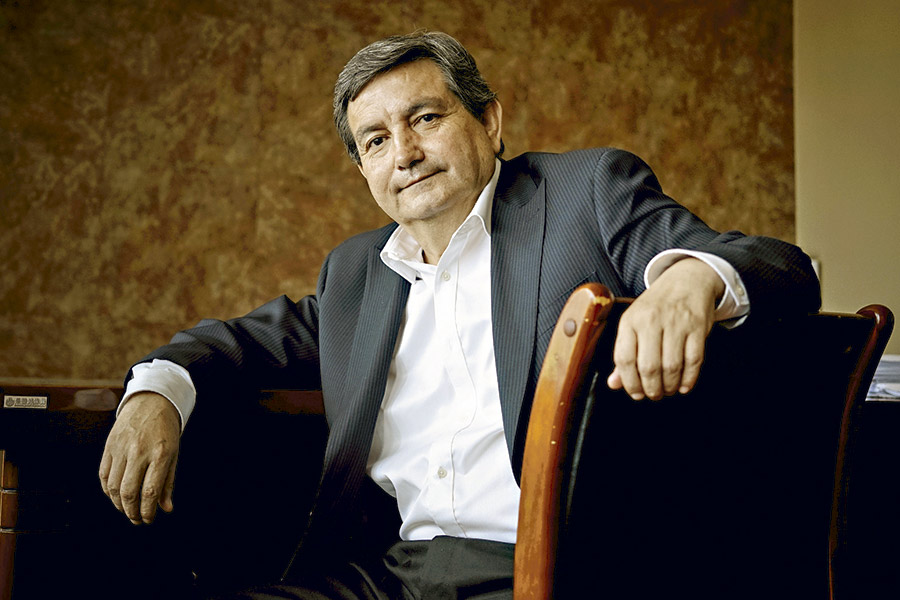
\includegraphics[width=0.4\textwidth]{figures/Miguel}
	\end{wrapfigure}
	Miguel Ángel Aguilera, ex-alcalde de San Ramón, enfrentó múltiples acusaciones relacionadas con enriquecimiento ilícito, lavado de activos y vínculos con el narcotráfico. Aguilera comenzó a ser investigado en 2017 tras reportes periodísticos que lo vinculaban con redes delictivas que operaban en la comuna. Durante su mandato, se detectaron millonarias inconsistencias entre sus ingresos declarados y su patrimonio, además de movimientos financieros sospechosos hacia cuentas personales y de terceros cercanos a su administración. Testimonios de exfuncionarios municipales señalaron que Aguilera mantenía un sistema de protección a personas involucradas en actividades ilegales, a cambio de beneficios económicos que se habrían utilizado para su enriquecimiento personal y campañas políticas.\cite{miguel}
	
	El caso tomó mayor relevancia cuando se descubrió que bienes raíces adquiridos por el exalcalde no coincidían con sus ingresos formales. Por ejemplo, propiedades registradas a su nombre en sectores exclusivos de Santiago y autos de lujo levantaron sospechas, generando una ola de indignación entre los vecinos de San Ramón. Adicionalmente, documentos filtrados mostraron adjudicaciones irregulares de contratos municipales a empresas ligadas a familiares y conocidos.
	
	\subsection{Análisis del caso}
	\subsubsection{Implicancias del caso}
	El caso de Miguel Ángel Aguilera pone de manifiesto la peligrosa infiltración del crimen organizado en las instituciones públicas. Más allá del daño económico, este tipo de corrupción afecta profundamente el tejido social al normalizar el desvío de recursos públicos y la protección de actividades ilícitas. La comuna de San Ramón, con altos índices de vulnerabilidad, se vio perjudicada al perder recursos destinados a mejorar servicios básicos como salud, educación e infraestructura.
	
	Además, este caso generó un precedente crítico para los órganos fiscalizadores. La falta de acción inmediata por parte de la Contraloría y otras instituciones permitió que Aguilera extendiera sus prácticas por años, consolidando un sistema corrupto en el municipio.
	
	\subsubsection{Estado actual del acusado}
	Aguilera fue formalizado en 2021 por delitos de lavado de activos y enriquecimiento ilícito. La Fiscalía logró demostrar que los montos involucrados superaban los 263 millones de pesos, además de identificar una red de colaboradores que facilitaron el ocultamiento de los fondos. Actualmente, el exalcalde se encuentra bajo arresto domiciliario total mientras se desarrolla el juicio oral. Los fiscales han solicitado una pena de 12 años de prisión, además de la confiscación de bienes adquiridos con recursos de origen ilícito.
	
	\subsubsection{Declaraciones}
	Miguel Ángel Aguilera ha defendido su inocencia, insistiendo en que las acusaciones son parte de una estrategia política para desprestigiarlo. Sin embargo, las pruebas presentadas por la Fiscalía, como transacciones bancarias, auditorías y testimonios, han debilitado su postura. En entrevistas previas, el exalcalde afirmó que su patrimonio era producto de ahorros familiares y negocios lícitos, aunque no presentó evidencia suficiente que respaldara estas afirmaciones.
	
	\section{Cuarto Caso}
	\begin{wrapfigure}{l}{0.4\textwidth}
		\centering
		
\includegraphics[width=0.4\textwidth]{figures/Karen}
	\end{wrapfigure}
	Karen Rojo, ex-alcaldesa de Antofagasta, fue condenada en 2022 por fraude al fisco tras descubrirse que utilizó fondos públicos para contratar a una consultora política con el objetivo de mejorar su imagen personal y asegurar su reelección. Durante su administración, entre 2015 y 2016, se desviaron más de 20 millones de pesos destinados a programas de desarrollo comunal hacia una empresa privada de coaching político. La investigación reveló que los contratos fueron elaborados sin las licitaciones correspondientes y ocultados bajo supuestas "asesorías técnicas".
	
	El caso generó un amplio rechazo público, especialmente en Antofagasta, donde los recursos malversados pudieron haber sido destinados a necesidades urgentes como el abastecimiento de agua y la mejora de infraestructura en escuelas locales. Además, las declaraciones de sus colaboradores, quienes admitieron haber firmado contratos bajo presión, dejaron en evidencia las prácticas irregulares dentro de su gestión.\cite{karen}
	
	\subsection{Análisis del caso}
	\subsubsection{Implicancias del caso}
	El caso de Karen Rojo es un ejemplo claro de cómo los recursos municipales pueden ser manipulados para fines personales, afectando directamente la confianza en las autoridades. La malversación de fondos destinados a proyectos esenciales impactó negativamente a los ciudadanos, quienes vieron sus necesidades desatendidas mientras los recursos se destinaban a campañas políticas.
	
	Este escándalo también resaltó fallas en los mecanismos de supervisión del gasto público. Las auditorías tardías y la permisividad en la elaboración de contratos fraudulentos permitieron que este esquema operara durante varios años sin ser detectado.
	
	\subsubsection{Estado actual del acusado}
	Karen Rojo fue condenada a cinco años y un día de cárcel. Inicialmente, escapó a Europa tras emitirse la sentencia, lo que provocó una orden de captura internacional. En 2022, fue detenida en Países Bajos y posteriormente extraditada a Chile para cumplir su condena. Actualmente, se encuentra en un centro penitenciario en Santiago, y se le han negado beneficios como la libertad vigilada debido al riesgo de fuga.
	
	\subsubsection{Declaraciones}
	Durante el proceso judicial, Rojo intentó justificar los pagos a la consultora como una medida para "optimizar la gestión municipal". Sin embargo, la evidencia presentada por la Fiscalía demostró que los servicios contratados tenían como objetivo exclusivo su campaña de reelección. En entrevistas recientes, Rojo ha evitado referirse directamente a los hechos y ha centrado su discurso en denunciar supuestas irregularidades en su proceso judicial.
	
	\section{Quinto Caso}
	\begin{wrapfigure}{r}{0.4\textwidth}
		\centering
		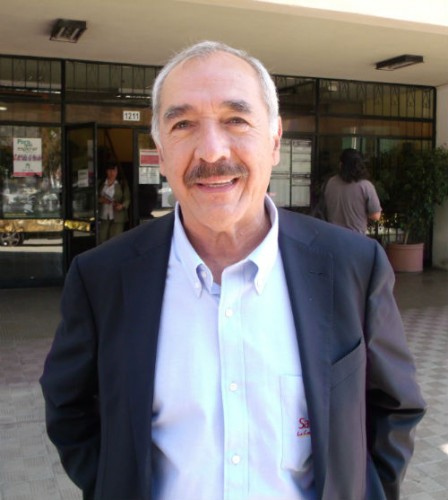
\includegraphics[width=0.4\textwidth]{figures/freire}
	\end{wrapfigure}
	Patricio Freire, ex-alcalde de San Felipe, fue formalizado por fraude al fisco, malversación de fondos y negociación incompatible. Durante su administración, entre 2014 y 2018, se detectaron múltiples irregularidades relacionadas con la adjudicación de contratos municipales a empresas vinculadas a familiares y personas de su círculo cercano. Estos contratos, destinados a proyectos de infraestructura pública, presentaron sobreprecios significativos y, en muchos casos, los proyectos no fueron ejecutados o quedaron abandonados. Según las investigaciones de la Fiscalía, los montos involucrados en estas irregularidades superaron los 300 millones de pesos.
	
	El esquema operado por Freire consistía en diseñar licitaciones a medida para garantizar que ciertas empresas fueran las únicas competidoras viables. Estas empresas, a menudo creadas recientemente o con experiencia limitada, presentaban propuestas con precios inflados que luego eran aprobadas sin mayor escrutinio. Entre los proyectos afectados destacan la construcción de un centro comunitario en el sector de Tierras Blancas, que nunca se inició, y la pavimentación de caminos rurales en la comuna, que quedó a medio terminar, afectando directamente a los habitantes de zonas apartadas.
	
	Adicionalmente, auditorías realizadas por la Contraloría General de la República descubrieron que algunos de los contratos adjudicados incluían cláusulas poco transparentes, como anticipos millonarios sin justificación técnica y la ausencia de garantías de cumplimiento. Estas prácticas no solo causaron un perjuicio económico a la comuna, sino que también generaron una crisis de confianza entre los ciudadanos y las autoridades locales.\cite{freire}
	
	\subsection{Análisis del caso}
	\subsubsection{Implicancias del caso}
	El caso de Patricio Freire evidencia la vulnerabilidad de los sistemas de contratación pública en las administraciones locales, particularmente en las comunas de menor tamaño donde los controles externos son menos frecuentes. La malversación de fondos destinados a proyectos críticos dejó a la comunidad de San Felipe sin acceso a servicios esenciales, como la mejora de caminos y espacios públicos, afectando principalmente a los sectores rurales.
	
	La corrupción en este caso también refleja un abuso sistemático del poder, donde los recursos públicos fueron utilizados para enriquecer a particulares en lugar de beneficiar a la comunidad. Esto perpetúa la percepción de impunidad en los cargos públicos y socava la confianza en las instituciones. En términos sociales, los habitantes de San Felipe, especialmente en los sectores más vulnerables, han expresado su indignación y frustración ante la falta de avances en proyectos prometidos durante la gestión de Freire.
	
	Además, el caso expone la falta de controles efectivos dentro del propio municipio. Los mecanismos de supervisión interna, como los departamentos de auditoría o control de contratos, no detectaron a tiempo las irregularidades, permitiendo que estas prácticas se consolidaran por varios años.
	
	\subsubsection{Estado actual del acusado}
	Actualmente, Patricio Freire se encuentra en prisión preventiva desde 2022 mientras se lleva a cabo el juicio oral. La Fiscalía ha solicitado una pena de ocho años de cárcel, considerando la magnitud del daño económico y la intencionalidad de los actos delictivos. Asimismo, se busca la devolución de los fondos malversados y la inhabilitación perpetua para ejercer cargos públicos, con el objetivo de evitar que el acusado pueda reincidir en actos similares.
	
	Paralelamente, las autoridades han iniciado procesos para recuperar los recursos desviados mediante la confiscación de bienes del acusado y de las empresas involucradas. Sin embargo, debido a la complejidad de rastrear el destino final de los fondos, se espera que este proceso sea prolongado. Además, la comunidad de San Felipe ha exigido la reactivación de los proyectos abandonados, aunque el municipio enfrenta limitaciones presupuestarias para retomar estas obras.
	
	\subsubsection{Declaraciones}
	En sus declaraciones públicas y judiciales, Patricio Freire ha negado todas las acusaciones, argumentando que los procesos de licitación se llevaron a cabo conforme a la normativa vigente y que las fallas en los proyectos se debieron a problemas técnicos y financieros ajenos a su responsabilidad. También ha intentado desviar la atención hacia sus supuestos logros como alcalde, mencionando iniciativas en áreas como educación y cultura.
	
	Sin embargo, los testimonios de exfuncionarios municipales han contradicho esta versión, señalando presiones directas por parte de Freire para adjudicar contratos a empresas específicas. Además, las auditorías de la Contraloría encontraron que muchos de los contratos adjudicados carecían de justificaciones técnicas y que las empresas beneficiadas estaban relacionadas con personas cercanas al exalcalde.
	
	Freire ha intentado posicionarse como una víctima de una persecución política, calificando las acusaciones como parte de una estrategia para desprestigiar su administración. No obstante, las pruebas documentales y los testimonios presentados en su contra han debilitado significativamente esta postura, dejando en evidencia un patrón sistemático de irregularidades durante su mandato.
	
	\subsubsection{Impacto en la comunidad}
	El caso ha tenido un impacto profundo en la percepción de la ciudadanía respecto a sus líderes locales. En particular, los sectores rurales, que dependían de los proyectos de infraestructura, han expresado su descontento a través de manifestaciones y peticiones formales para que se acelere el juicio y se reanuden las obras inconclusas. Además, el desprestigio del municipio ha afectado su capacidad de atraer inversiones externas, complicando aún más la recuperación económica de la comuna.
	
	En conclusión, el caso de Patricio Freire es un ejemplo emblemático de cómo la corrupción puede afectar negativamente a las comunidades, no solo en términos económicos, sino también sociales y políticos. Este caso resalta la necesidad de fortalecer los sistemas de fiscalización y control en las administraciones locales para prevenir abusos similares en el futuro.
	
	\section{Conclusión}
	
	El análisis de los casos de corrupción municipal en Chile demuestra la gravedad y el impacto que estos actos tienen sobre las comunidades locales. Los delitos cometidos por alcaldes como Margarita Osorio, Óscar Cortés, Miguel Ángel Aguilera, Karen Rojo y Patricio Freire no solo representan un perjuicio económico significativo, sino que también erosionan la confianza ciudadana en las instituciones públicas. Estos casos ponen de manifiesto la fragilidad de los sistemas de fiscalización y control, permitiendo que abusos de poder y desvíos de recursos queden impunes durante años.
	
	Una constante en los casos estudiados es la vulnerabilidad de las comunidades más necesitadas frente a estas prácticas corruptas. Los fondos malversados estaban destinados a proyectos esenciales como viviendas, infraestructura, y servicios básicos, dejando a muchas familias en situación de desamparo. Además, estos actos perpetúan un ciclo de desconfianza, debilitando la relación entre las autoridades locales y la ciudadanía, e impactando negativamente el desarrollo de las comunas afectadas.
	
	Es evidente la necesidad de fortalecer los mecanismos de supervisión y sanción en la administración pública. Esto incluye la implementación de auditorías más rigurosas, el uso de tecnología para garantizar la transparencia en las licitaciones y contratos, y la promoción de una cultura de honradez entre los funcionarios públicos. Asimismo, es crucial que las penas aplicadas sean ejemplares, para disuadir futuros actos de corrupción y garantizar que quienes cometan estos delitos enfrenten las consecuencias legales correspondientes.
	
	Finalmente, la participación activa de la ciudadanía y de los medios de comunicación juega un rol fundamental en la denuncia de irregularidades y en la exigencia de rendición de cuentas por parte de las autoridades. Solo a través de un esfuerzo conjunto entre el gobierno, las instituciones fiscalizadoras y la sociedad comunal será posible combatir la corrupción y reconstruir la confianza en los gobiernos locales.
	
	
	\newpage
	\printbibliography[heading=bibintoc, title=Referencias]
	
\end{document}